% ---------- Titelblad Masterproef Faculteit Wetenschappen -----------
% Dit document is opgesteld voor compilatie met pdflatex.  Indien je
% wilt compileren met latex naar dvi/ps, dien je de figuren naar
% (e)ps-formaat om te zetten.
%                           -- december 2012
% -------------------------------------------------------------------
\RequirePackage{fix-cm}
\documentclass[12pt,a4paper,oneside]{book}

% --------------------- In te laden pakketten -----------------------
% Deze kan je eventueel toevoegen aan de pakketten die je al inlaadt
% als je dit titelblad integreert met de rest van thesis.
% -------------------------------------------------------------------
\usepackage{graphicx,xcolor,textpos}
\usepackage[utf8]{inputenc}
\usepackage[T1]{fontenc}
\usepackage{helvet}
\usepackage{amsmath}
\usepackage{hyperref}
\usepackage[hypcap]{caption}
\usepackage{listings}
\usepackage{color}

% -------------------- Pagina-instellingen --------------------------
% Indien je deze wijzigt, zal het titelblad ook wijzigen.  Dit dien je
% dan manueel aan te passen.
% --------------------------------------------------------------------
\topmargin -10mm
\textwidth 160truemm
\textheight 240truemm
\oddsidemargin 0mm
\evensidemargin 0mm

% ------------------- textpos-instellingen ---------------------------
% Enkele andere instellingen voor het voorblad.
% --------------------------------------------------------------------
\definecolor{green}{RGB}{172,196,0}
\definecolor{bluetitle}{RGB}{29,141,176}
\definecolor{blueaff}{RGB}{0,0,128}
\definecolor{blueline}{RGB}{82,189,236}
\definecolor{dkgreen}{rgb}{0,0.6,0}
\definecolor{gray}{rgb}{0.5,0.5,0.5}
\definecolor{mauve}{rgb}{0.58,0,0.82}
\setlength{\TPHorizModule}{1mm}
\setlength{\TPVertModule}{1mm}

% Eigen instellingen
\renewcommand{\contentsname}{Inhoud}
\renewcommand{\listfigurename}{Lijst van figuren}
\renewcommand{\listtablename}{Lijst van tabellen}
\renewcommand{\chaptername}{Hoofdstuk}
\renewcommand{\chapterautorefname}{hoofdstuk}
\renewcommand{\sectionautorefname}{sectie}
\renewcommand{\subsectionautorefname}{sectie}
\renewcommand{\figureautorefname}{figuur}

\lstset{frame=tb,
  language=Java,
  aboveskip=3mm,
  belowskip=3mm,
  showstringspaces=false,
  columns=flexible,
  basicstyle={\small\ttfamily},
  numbers=left,
  numberstyle=\tiny\color{gray},
  keywordstyle=\color{blue},
  commentstyle=\color{dkgreen},
  stringstyle=\color{mauve},
  breaklines=true,
  breakatwhitespace=true,
  tabsize=4,
  escapechar=|
}

\begin{document}

% ---------------------- Voorblad ------------------------------------
% Vergeet niet de tekst aan te passen:
% - Titel en, indien van toepassing, ondertitel
%          voor eventuele formules in de titel of ondertitel
%          gebruik je  \form{$...$}
% - Je naam
% - Je (co)promotor, begeleider (indien van toepassing)
% - Je opleiding
% - Het academiejaar
% --------------------------------------------------------------------
\thispagestyle{empty}
\newcommand{\form}[1]{\scalebox{1.087}{\boldmath{#1}}}
\sffamily
%
\begin{textblock}{191}(-24,-11)
\colorbox{green}{\hspace{123mm}\ \parbox[c][18truemm]{68mm}{\textcolor{white}{FACULTEIT WETENSCHAPPEN}}}
\end{textblock}
%
\begin{textblock}{70}(-18,-19)
\textblockcolour{}
\includegraphics*[height=19.8truemm]{LogoKULeuven.png}
\end{textblock}
%
\begin{textblock}{79}(50,50)
\centerline{\includegraphics*[height=10.0truecm]{voorbladpacking.png}}
%De achtergrond kan wit blijven of je kan een afbeelding invoegen (maximum hoogte 10 cm, breedte variabel, denk aan auteursrechten\ldots). GEEN logo's (je kan binnenin de masterproef logo's gebruiken, maar niet op de voor- of achterpagina).
\end{textblock}
%
\begin{textblock}{160}(-6,63)
\textblockcolour{}
\vspace{-\parskip}
\flushleft
\fontsize{40}{42}\selectfont \textcolor{bluetitle}{Een nieuwe constructieve heuristic voor het plaatsen van cirkels in een cirkel}\\[1.5mm]
\fontsize{20}{22}\selectfont Gebaseerd op een \textit{best-fit} methodiek
\end{textblock}
%
\begin{textblock}{160}(8,153)
\textblockcolour{}
\vspace{-\parskip}
\flushright
\fontsize{14}{16}\selectfont \textbf{Pablo BOLLANSÉE}
\end{textblock}
%
\begin{textblock}{70}(-6,191)
\textblockcolour{}
\vspace{-\parskip}
\flushleft
Promotor: Prof. P. De Causmaecker \\[-2pt]
\textcolor{blueaff}{Affiliatie \textsl{(facultatief)}}\\[5pt]
Co-promotor: \textsl{(facultatief)}\\[-2pt]
\textcolor{blueaff}{Affiliatie \textsl{(facultatief)}}\\[5pt]
Begeleider: \textsl{(facultatief)}\\[-2pt]
\textcolor{blueaff}{Affiliatie \textsl{(facultatief)}}\\
\end{textblock}
%
\begin{textblock}{160}(8,191)
\textblockcolour{}
\vspace{-\parskip}
\flushright
Proefschrift ingediend tot het\\[4.5pt]
behalen van de graad van\\[4.5pt]
Master of Science in de\\[4.5pt]
toegepaste informatica\\
\end{textblock}
%
\begin{textblock}{160}(8,232)
\textblockcolour{}
\vspace{-\parskip}
\flushright
Academiejaar 2015-2016
\end{textblock}
%
\begin{textblock}{191}(-24,248)
{\color{blueline}\rule{550pt}{5.5pt}}
\end{textblock}
%
\vfill

\newpage
\thispagestyle{empty}
\begin{textblock}{160}(0,185)
© Copyright by KU Leuven

Zonder voorafgaande schriftelijke toestemming van zowel de promotor(en) als de auteur(s) is overnemen, kopiëren, gebruiken of realiseren van deze uitgave of gedeelten ervan verboden. Voor aanvragen tot of informatie i.v.m. het overnemen en/of gebruik en/of realisatie van gedeelten uit deze publicatie, wendt u tot de KU Leuven, Faculteit Wetenschappen, Geel Huis, Kasteelpark Arenberg 11 bus 2100, 3001 Leuven (Heverlee), Telefoon +32 16 32 14 01.

Voorafgaande schriftelijke toestemming van de promotor(en) is eveneens vereist voor het aanwenden van de in dit afstudeerwerk beschreven (originele) methoden, producten, schakelingen en programma’s voor industrieel of commercieel nut en voor de inzending van deze publicatie ter deelname aan wetenschappelijke prijzen of wedstrijden.
\end{textblock}

\newpage

% Als je het titelblad wil integreren met de rest van je thesis,
% kan je hieronder verder.
% ----------------------- Eerste pagina's -------------------------
% Hier kan je inhoudsopgave, voorwoord en dergelijke kwijt.
% -----------------------------------------------------------------
\rmfamily
\setcounter{page}{0}
\pagenumbering{roman}

\newpage

\chapter*{Voorwoord}
\addcontentsline{toc}{chapter}{Voorwoord}

Het circle-packing probleem bestaat er uit om een aantal cirkels, met gekende radii, in een zo klein mogelijke container te plaatsen.
De vorm van deze container kan verschillen, meestal is het een driehoek, rechthoek of cirkel.
In deze thesis stel ik een nieuwe \textit{best-fit} gebaseerde heuristiek voor voor het plaatsen van cirkels in een cirkel.
Het is een constructieve heuristiek waarin stapsgewijs telkens de best-passende cirkel geplaatst zal worden.

Wiskundig is dit een relatief eenvoudig probleem om voor te stellen, maar computationeel is het zeer zwaar om exact op te lossen.
Bestaande pogingen om dit probleem op te lossen vragen zeer veel tijd om het te berekenen.
In deze thesis stel ik een nieuwe heuristiek voor die het mogelijk maakt zéér snel oplossingen te genereren.

Ik wil hierbij Patrick De Causmaeker bedanken voor alle hulp en ondersteuning bij het ontwerpen van deze heuristiek en verwezenlijken van dit werk.
Ook wil ik Jim Bollansée en Marie Julia Bollansée bedanken voor hun hulp bij het schrijven van deze tekst.

%  In het voorwoord wordt de algemene doelstelling van het werk samengevat
%  in enkele regels en worden personen, diensten of firma’s bedankt voor hun
%  medewerking bij het tot stand komen van het werk.
%  De naam van firma’s en personen uit deze firma’s mogen slechts worden vermeld
%  mits hun uitdrukkelijke toelating én na overleg met de supervisor(en)! Steeds
%  wordt de supervisor(en) vermeld, de verantwoordelijke en eventueel de personen
%  die rechtstreeks geholpen hebben bv. door het ter beschikking stelling van
%  meetresultaten, faciliteiten. Ook de instantie die eventueel een doctoraatsbeurs
%  heeft toegekend wordt bedankt (bv. FWO, IWT, . . . ).

\newpage

\chapter*{Abstract}
\addcontentsline{toc}{chapter}{Abstract}

TODO

%  In een beknopte tekst van maximum 2 pagina’s worden de belangrijkste
%  doelstellingen en besluiten geformuleerd, zowel in het Nederlands als in het
%  Engels. Zulke samenvattingen kunnen worden gebruikt in wetenschappelijke
%  verslagen van het departement of de faculteit. Het Engels moet vlekkeloos zijn.

\newpage

\tableofcontents
\listoffigures
\addcontentsline{toc}{chapter}{Lijst van figuren}
\listoftables
\addcontentsline{toc}{chapter}{Lijst van tabellen}

\newpage

% ----------------------- Eigenlijke thesis -----------------------
% Vanaf de inleiding/het eerste hoofdstuk.
% -----------------------------------------------------------------
\setcounter{page}{0}
\pagenumbering{arabic}

\chapter{Inleiding}

In deze thesis stel ik een nieuwe \textit{best-fit} gebaseerde heuristiek voor voor het cirkle-packing probleem.
De heuristiek is specifiek voor sub-probleem van het plaatsen van cirkels in een cirkel.
Ook bespreek ik de implementatie die gemaakt is naast de ontwikkeling van de heuristiek.
Dit circle-packing probleem bestaat uit het plaatsen van $n$ cirkels in een zo klein mogelijke cirkelvormige container.
Het is de bedoeling om voor de gegeven cirkels de coordinaten van de middelpunten te vinden zodat deze niet overlappen en de radius van de omcirkel zo klein mogelijk is.

Circle-Packing is zowel theoretisch als practisch een zeer interessant probleem.
Het kan gebruikt worden om verschillende real-world problemen op te lossen, zoals het plaatsen van zendmasten, stokage van cilindrische voorwerpen, en het combineren van verschillende kabels.

Mathematisch is het redelijk eenvoudig als een optimalisatie probleem te omschrijven:

\begin{equation*}
\begin{aligned}
& \text{minimaliseer}
& & r \\
& \text{onderhevig aan}
& & x_i^2 + y_i^2 \leq (r-r_i)^2, 
& & &i = {1,...,n}\\
&&& (x_i - x_j)^2 + (y_i + y_j)^2 \geq (r_i + r_j)^2,
& & &i \neq j
\end{aligned}
\end{equation*}

Hierin is $r_i$ de radius, en $(x_i,y_i)$ de coördinaten van het centrum van cirkel $i$.
Hierbij wordt verondersteld dat de omcirkel het nulpunt als middelpunt heeft.
De eerste formule verzekerd dat de cirkels in de omcirkel liggen, en de tweede dat ze elkaar niet overlappen.
In het geval dat alle cirkels de zelfde grootte hebben wordt meestal $r_i$ altijd gelijk aan $1$ genomen.
Het circle-packing probleem voor andere containers heeft gelijkaardige, relatief eenvoudige, wiskundige omschrijvingen.

Hoewel dit wiskundig zeer eenvoudig te omschrijven is, blijft het toch een zeer moeilijk probleem om exact op te lossen.
Het is een NP-hard probleem.
Daarom zoekt men naar andere technieken om het toch op te kunnen lossen.
Er is reeds veel onderzoek gebeurt naar het oplossen van het circle-packing probleem voor zowel cirkels van gelijke gootte, als voor cirkels van verschillende grootte.
In \cite{graham1996repeated} en \cite{lubachevsky1997curved} probeert men vaste patronen te vinden die een optimale packing van cirkels met gelijke grootte geeft.
In \cite{graham1998dense}, \cite{lubachevsky1991simulate} en \cite{wang2002improved} worden fysisch geïnspireerde simulaties gebruikt om packing te bekomen.
Ook worden zijn er pogingen om meta-heuristieken te gebruiken om packings te bekomen.
In \cite{george1995packing} worden verschillende meta-heuristieken, waaronder een genetisch algoritme, uitgeprobeerd en vergeleken.
Zij ondervinden dat dit genetisch algoritme en een quasi-random techniek, in vergelijking met de andere uitgeprobeerde meta-heuristieken, de beste resultaten geven.
In \cite{hifi2004approximate} en \cite{hifi2004simulated} worden respectievelijk een genetisch en een simulated-annealing algoritme voorgesteld.
Een recentere poging is het Monotonic Basin Hopping algoritme voorgesteld in \cite{grosso2010}.
Hierin beschrijven ze dat er teveel lokale optima zijn voor een eenvoudige multi-start behandeling, en stellen een variant voor waarin ze op een slimme manier de begin punten proberen genereren.
Ook relatief recent is \cite{jors2011}, waarin gebruik wordt gemaakt van de combinatorische eigenschappen van circle-packing in combinatie met een taboo-search en een off-the-shelf non-linear optimizer.
Hierin plaatsen ze één voor één elke cirkel en laat de non-linear optimizer hiervoor telkens een lokaal extremum berekenen.
Ze zoeken van met de taboo-search naar de beste volgorde om de cirkels te plaatsen.

Constructieve algoritmen voor het oplossen van circle-packings zijn veel minder onderzocht.
Eén van de weinig constructieve methoden word beschreven in \cite{akeb2006basic}, waar ze een alternatieve vorm van circle-packings oplossen: de grootte van de container ligt vast, en je moet zo veel mogelijk cirkels van gelijke grootte er in plaatsen.
In \cite{hifi2004approximate} wordt er dan weer een aanpassing gedaan op de klassieke bottom-left-first heuristiek, voor het plaatsen van rechthoeken, om gebruikt te maken van de cirkelvormigheid van de objecten.

Hoewel veel van deze oplossingen zeer goede packings maken, regelmatig verbeteren ze hun voorganger, vragen ze zeer veel reken tijd en beperken ze zich tot een klein aantal cirkels.
In deze thesis stel ik een nieuw constructieve heuristiek voor om het circle-packing probleem op te lossen.
Deze laat toe in een fractie van de tijd nodig voor andere algoritmen packings te maken.
Ook is het mogelijk om veel grotere aantallen cirkels te plaatsen.
De packings zijn echter minder dicht dan deze verkregen in voorgenoemd onderzoek.
Deze \textit{verslechtering} blijft echter beperkt en laat toe de packings in slecht enkele ogenblikken te maken, waar anderen uren rekentijd vragen.

De heuristiek voorgesteld in deze thesis is een best-fit heuristiek gebaseerd op een oplossing voor het Orthogonal Stock-Cutting Problem voorgesteld in \cite{burke2004new}.
Zij stellen een heuristiek voor die de volgende balk om te plaatsen kiest uit een lijst, en deze plaatst op de \textit{beste} positie.
Dit in tegenstelling tot cirkels plaatsen in een vooraf bepaalde volgorde zoals in \cite{grosso2010} en \cite{jors2011}.
Op een gelijkaardige manier kiest mijn algoritme de volgende cirkel die best past in de huidige packing.

In \autoref{chap:algoritme} bespreek ik hoe de heuristiek opgebouwd is.
Ik bespreek de twee basis concepten voor mijn best-fit heuristiek: \textit{holes} en de \textit{shell}.
Ik bespreek hoe deze werken, en op welke manier gekozen wordt welke cirkel best past in de packing.
Hierbij bespreek ik ook de implementatie. In \autoref{chap:resultaten} worden de verkregen resultaten besproken.
Hier vergelijk ik de packings met de best gekende resultaten zoals gerapporteerd op de Packomania website (\cite{packomania}).
Ik doe hier een vergelijking zowel op omtrek van de verkregen omcirkel, als op nodige tijd om deze packing te berekenen tegenover de best gekende oplossingen.
Ook toon ik resultaten voor packings voor veel meer cirkels dan getoond op de Packomania website.
In \autoref{chap:opmerkingen-en-verder-werk} bespreek ik mogelijke verbeteringen, de \textit{losse eindjes} en ideeën voor verdere uitbreidingen en onderzoek.
In \autoref{chap:handleiding-visualisaties} wordt kort verduidelijkt hoe u de visualisaties gebruikt doorheen deze thesis kan interpreteren.

\chapter{Handleiding voor het lezen van de visualisaties} \label{chap:handleiding-visualisaties}

Doorheen deze thesis zal ik gebruik maken visualisaties gegenereerd door de java implementatie van het algoritme.
Dit om de concepten grafisch te verduidelijken.
Twee voorbeelden van zulke visualisaties zijn \autoref{fig:handleiding-visualisatie-1} en \autoref{fig:handleiding-visualisatie-2}.

\begin{figure}
  \centering
  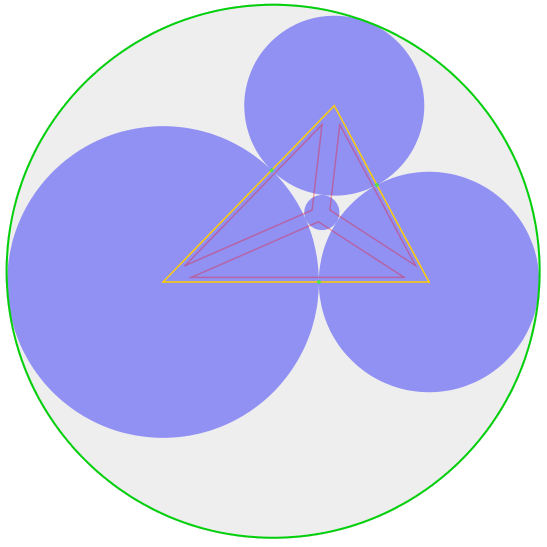
\includegraphics[width=0.65\textwidth]{handleiding-visualisatie-1.png}
  \caption{Voorbeeld visualisatie met drie duidelijke holes} \label{fig:handleiding-visualisatie-1}
\end{figure}

\begin{figure}
  \centering
  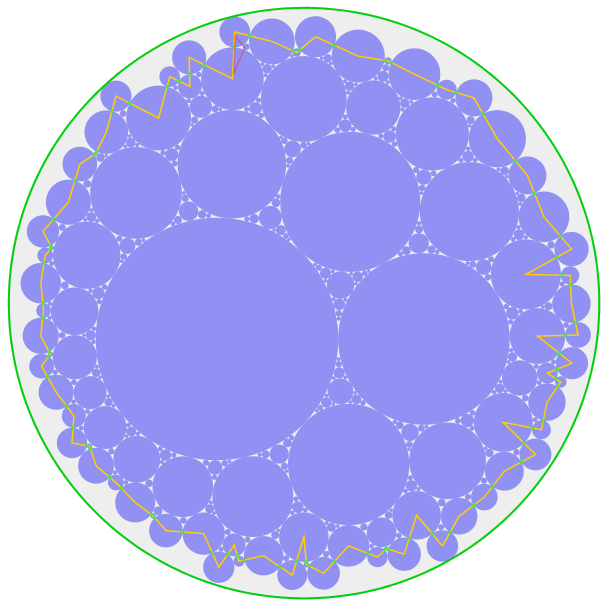
\includegraphics[width=0.65\textwidth]{handleiding-visualisatie-2.png}
  \caption{Voorbeeld visualisatie met grote shell} \label{fig:handleiding-visualisatie-2}
\end{figure}

Deze figuren kan u op de volgende manier interpreteren:

\begin{itemize}  
\item De \textbf{reeds geplaatste cirkels} worden getoond als \textbf{licht blauwe cirkels}.
\item De \textbf{shell} is een \textbf{gele lijn} aan de buitenste rand van de packing.
\item De kleine \textbf{groene bolletjes} op de shell geven de posities aan waarop mogelijk een cirkel geplaatst zal worden.
\item \textbf{Holes} worden getoond als \textbf{rode driehoeken}.
\item De \textbf{omcirkel} van de huidige packing wordt getoond als een \textbf{groene cirkel}.
\end{itemize}

Op \autoref{fig:handleiding-visualisatie-1} is zijn er duidelijk drie holes te zien.
Elk van de drie holes word gedefinieerd door de centrale cirkel en twee van de buitenste cirkels.
Ook is er een kleine shell te zien, die bestaat uit de buitenste drie cirkels.
In \autoref{fig:handleiding-visualisatie-2} wordt een verder gevorderde packing getoond waarop één hole te zien is, en een veel grotere shell.
Op beide figuren kan je ook de omcirkel zien.

\chapter{Algoritme} \label{chap:algoritme}

In dit hoofdstuk bespreek ik de werking van de heuristiek.
Eerst geef ik een korte beschrijving van het basis idee van het algoritme, gevolgd door de structuur van de code.
Vervolgens leg ik stelselmatig de volledige werking uit, alle veronderstellingen die gemaakt worden en implementatie details waar nodig.
De volledige implementatie is beschikbaar op GitHub \cite{circle-packing-github} en in gebeurt in Java.

\section{Basis idee}

Het basis idee van de heuristiek is om stelselmatig een packing op te bouwen, door telkens cirkels te zoeken die het best passen.
Bij elke stap wordt telkens eerst een plek gekozen wordt om een cirkel te plaatsen (in een hole, of op de shell, later hier meer over).
Hier wordt dan de best-passende cirkel geplaatst.
Eenmaal een cirkel geplaatst is wordt deze nooit meer verplaatst.
Dit laat toe om intelligente structuren op te bouwen en deze op een zeer efficiënte manier te gebruiken.

Het algoritme bouwt dus cirkel per cirkel een packing op.
Dit door in elke stap een positie te kiezen, en hierin een cirkel te proberen plaatsen.
Indien er geen cirkel geplaatst kan worden wordt de interne structuur van het probleem vernieuwd om deze nieuwe informatie te reflecteren.
Dit gebeurt op verschillende manieren voor de holes en de shell.
Meer hierover vindt u terug in \autoref{sec:holes} en \autoref{sec:shell}.
Als er wel een cirkel geplaatst kan worden dan wordt deze uit de lijst van nog-te-plaatsen cirkels verwijderd, en krijgt deze een permanente positie daar.
Dit geeft ook aanleiding tot aanpassen van de holes en/of shell.
Hierdoor wordt er een nieuwe tussentijdse packing gemaakt.
Deze wordt dan door gegeven naar de volgende stap, waarin het algoritme opnieuw zal proberen een cirkel te plaatsen.
Op deze manier word een volledige packing opgebouwd voor alle cirkels.

\section{Structuur}

De implementatie van het algoritme is op te delen in drie belangrijke delen.

\begin{itemize}  
\item Problem of probleem
\item Solution of oplossing
\item Solver of oplosser
\end{itemize}

Bovenop deze delen komen dan ook nog enkele voor de hand liggende hulp klassen, zoals $circle$ en $vector2$.
Ook zijn er klassen voorzien om de uiteindelijke oplossing te visualiseren, tussen stappen te visualiseren en automatisch verschillende tests uit te voeren.

Een $problem$ of probleem is een lijst van cirkels.
Deze hebben nog geen positie, en worden gesorteerd van groot naar klein.
Dit is wat de $solver$ als input krijgt.

Een $solution$ of oplossing is een lijst van cirkels met hun positie.
Dit kan een tussen oplossing zijn, waar nog niet voor alle cirkels uit een probleem een positie gevonden is.
Ook geeft dit geen garanties van correctheid, er kan dus bijvoorbeeld overlap zijn, maar voorziet functionaliteit om dit na te gaan.
Dit is wat de solver als output geeft.
Een correcte solver geeft natuurlijk wel altijd goede oplossingen.

Een $solver$ of oplosser is het object dat een packing zoekt voor een gegeven probleem.
Dit is dus het belangrijkste deel van de code, en hier is de nieuwe heuristiek geïmplementeerd.
De best-fit solver, zoals beschreven in deze thesis, doet dit stap voor stap.
In elke stap wordt er één cirkel geplaats op zijn finale positie, dit aan de hand van enkele keuzes die verder in dit hoofdstuk toegelicht zullen worden.


\section{Structuur van de solver}

Zoals hierboven gezegd is de solver het hart van de implementatie.
Deze maakt effectief een packing voor een gegeven probleem.
De solver bevat een lijst van \textit{holes} en de \textit{shell}.
Het bevat ook een lijst van de nog te plaatsen cirkels, en een tussen-oplossing met de cirkels die reeds een plaats gekregen hebben.
Ook heeft hij interne omcirkel voor deze oplossing.
Een oplossing kan zelf ook een omcirkel berekenen, maar de solver gebruikt een interne omcirkel die enkel vernieuwd wordt als het nodig is.
Bovendien heeft de solver extra informatie die de oplossing niet heeft, waardoor deze omcirkel efficiënter berekend kan worden.
Zie \autoref{chap:shell} voor meer uitleg hierover.

De best-fit solver uit deze thesis kan stap voor stap de oplossing genereren.
Dit zorgt er voor dat tussentijdse stappen gevisualiseerd kunnen worden.
Het is dus niet nodig een packing volledig te maken, het kan zeer nuttig zijn tussentijdse packings te zien, zeker bij het debuggen of implementeren van nieuwe functionaliteit.

//TODO Code best-fit-step?

\section{Initialisatie}

Zoals eerder gezegd bouwt het algoritme steeds verder op een packing uit de vorige stap.
Hierdoor is het dus nodig om een initiële packing te maken van een aantal cirkels waarop de volgende stappen kunnen verder bouwen.
Deze initiële packing is eenvoudigweg een packing van de drie grootste cirkels in het probleem.
Deze drie cirkels worden zo geplaatst dat ze alle drie aan elkaar raken, zoals getoond in \autoref{fig:initialisatie}.
De licht blauwe cirkels tonen de drie eerste-geplaatste cirkels.
Meer uitleg over hoe u deze figuur kan interpreteren kan u vinden in \autoref{chap:handleiding-visualisaties}

\begin{figure}
  \centering
  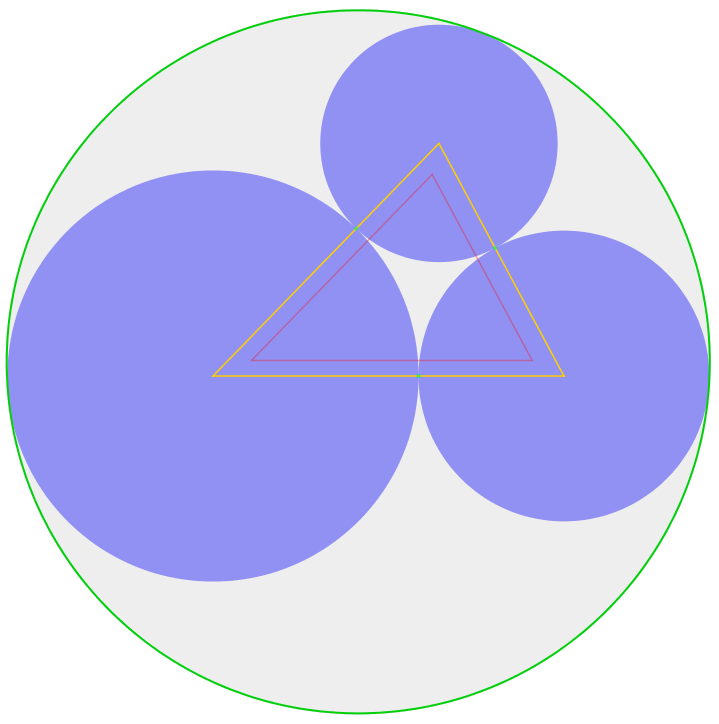
\includegraphics[width=0.65\textwidth]{initialisatie.png}
  \caption{Voorbeeld van initiële packing} \label{fig:initialisatie} 
\end{figure}

// TODO Interessant om deze code toe te voegen?

\begin{lstlisting}
	private void packFirstThree() {
		//Initially place the two biggest circles next to eachother
		Circle first = circlesToPack.get(0);
		Circle second = circlesToPack.get(1);

		Vector2 firstPos = new Vector2(0, 0);
		Vector2 secondPos = new Vector2(first.getRadius() + second.getRadius(), 0);

		Location firstLoc = new Location(firstPos, first);
		Location secondLoc = new Location(secondPos, second);

		getSolution().add(firstLoc);
		getSolution().add(secondLoc);

		// Place the third biggest circle on top of the first two (assuming they are positioned clockwise)
		Circle third = circlesToPack.get(2);
		Vector2 thirdPos = Helpers.getMountPositionFor(third, firstLoc, secondLoc);
		Location thirdLoc = new Location(thirdPos, third);
		getSolution().add(thirdLoc);

		circlesToPack.remove(first);
		circlesToPack.remove(second);
		circlesToPack.remove(third);

		// Create first hole
		holes.add(new NHole(firstLoc, secondLoc, thirdLoc));
		// Create the initial shell
		// IMPORTANT: must be clock-wise
		shell.add(firstLoc);
		shell.add(thirdLoc);
		shell.add(secondLoc);

		enclosingCircle = Location.calculateEnclosingCircle(Arrays.asList(firstLoc, secondLoc, thirdLoc));
	}
\end{lstlisting}

// TODO Licht de code toe

\section{Holes} \label{sec:holes}

Het eerste van de twee belangrijkste concepten van de heuristiek is \textit{holes} of \textit{gaten}.
Dit zijn plaatsen tussen andere, reeds geplaatste, cirkels waar potentieel nog een cirkel tussen kan passen.
De heuristiek zal telkens eerst deze gaten proberen op te vullen, alvorens cirkels op de shell te plaatsen.

Gaten worden gedefinieerd door exact drie cirkels in de huidige packing.
De solver houdt informatie bij voor elk gat waar mogelijk nog een cirkel in kan passen.
Bij elke stap van de solver zal er eerst gekeken worden of er nog gaten in de oplossing zijn.
Indien er nog gaten zijn zal hij deze dus eerst hier een cirkel in proberen plaatsen.
Indien het gat te klein is voor alle nog-te-plaatsen cirkels wordt dit gat simpelweg verwijderd uit de lijst van gaten in de solver.
Op deze manier weet de solver in de volgende stap dat hij daar niet meer moet proberen om een cirkel te plaatsen, en zal hij een ander gat uitproberen.
Indien er wel een cirkel in het gat past wordt deze daar in geplaatst.
Dit zal leiden tot het creëren van drie nieuwe gaten, zoals getoond in ... en ....

// TODO Voeg twee afbeeldingen toe, eerste van een gat, tweede waarin het gat opgevuld is en aanleiding geeft tot 3 nieuwe gaten.

\subsection{Grootste cirkel zoeken die past een \textit{hole}}

Bij het plaatsen van een cirkel in een gat wordt een zo groot mogelijke cirkel gezocht die in dit gat past.
Dit is bij wijze van spreken de best-passende cirkel, vandaar \textit{best-fit}.
Meer uitleg over hoe bepaald wordt of een cirkel past vind je in \autoref{subsec:bepalen-of-een-cirkel-past-in-hole}.
Er wordt logaritmisch gezocht door de lijst van cirkels om te bepalen welke cirkel de grootste is die past.
De solver houdt de lijst van cirkels bij gesorteerd op grootte, dat is cruciaal om snel de beste-passende cirkel te vinden.
Eerst worden de grootste en kleinste cirkel uitgeprobeerd.
Indien de kleinste niet past zal het algoritme direct rapporteren dat dit gat te klein is.
Het gat zal dan, zoals vermeld in \autoref{sec:holes}, verwijderd worden uit de lijst van mogelijk holes.
Indien de grootste past zal het algoritme onmiddellijk deze cirkel plaatsen in het gat.
Er zijn immers geen grotere cirkels, dus deze is de cirkel die verondersteld wordt best te passen.
Vervolgens word er een gebied bepaald in de overblijvende cirkels, waarin de best-passende cirkel zich bevind.
Initieel ligt de boven-en ondergrens van dit gebied op de uiteinden van de overblijvende cirkels.
De cirkel in de midden van dit gebied wordt dan uitgeprobeerd.
Afhangende of deze wel of niet past zal de boven-of ondergrens aangepast worden.
Dit wordt telkens herhaald tot er nog maar één cirkel over blijft.
Dit is dan de grootste cirkel die past in het gat.

// TODO Add code

\subsection{Bepalen of een cirkel past in een \textit{hole}} \label{subsec:bepalen-of-een-cirkel-past-in-hole}

Er is geen exact definitie van de grootte van een gat.
Dit is niet mogelijk omdat de cirkels die het gat bepalen niet altijd aan elkaar raken.
Het is echter wel mogelijk om te bepalen of een cirkel past.
Dit gebeurt door de cirkel $c_i$, met radius $r_i$, die je wilt testen te plaatsen zodat hij twee van de drie cirkels $c_g1, c_g2$, met radii $r_g1, r_g2$, van het gat raakt.
Het punt vinden waarop deze cirkel moet staan om beide andere cirkels te raken wordt bepaald door een eenvoudige cirkel-cirkel intersectie, tussen twee cirkels met hun middelpunt gelijk aan het middelpunt van de cirkels $c_g1$ en $c_g2$ en als radii $r_g1+r_i$ en $r_g2+r_i$:

\begin{lstlisting}
	Vector2 getMountPositionFor(Circle cir, Location first, Location second) {
		double x0 = first.getPosition().getX();
		double y0 = first.getPosition().getY();
		double r0 = first.getCircle().getRadius() + cir.getRadius();

		double x1 = second.getPosition().getX();
		double y1 = second.getPosition().getY();
		double r1 = second.getCircle().getRadius() + cir.getRadius();

		/* dx and dy are the vertical and horizontal distances between
		 * the circle centers.
		 */
		double dx = x1 - x0;
		double dy = y1 - y0;

		/* Determine the straight-line distance between the centers. */
		//d = sqrt((dy*dy) + (dx*dx));
		double d = Math.hypot(dx, dy);

		/* 'point 2' is the point where the line through the circle
		 * intersection points crosses the line between the circle
		 * centers.
		 */

		/* Determine the distance from point 0 to point 2. */
		double a = ((r0*r0) - (r1*r1) + (d*d)) / (2.0 * d) ;

		/* Determine the coordinates of point 2. */
		double x2 = x0 + (dx * a/d);
		double y2 = y0 + (dy * a/d);

		/* Determine the distance from point 2 to either of the
		 * intersection points.
		 */
		double h = Math.sqrt((r0*r0) - (a*a));

		/* Now determine the offsets of the intersection points from
		 * point 2.
		 */
		double rx = -dy * (h/d);
		double ry = dx * (h/d);

		/* Determine the absolute intersection points. */
		return new Vector2(x2 - rx, y2 - ry);
	}
\end{lstlisting}
// TODO Is deze code interessant?

Een cirkel-cirkel intersectie heeft natuurlijk altijd twee punten.
Hiervan moet er één gekozen worden.
Door systematisch de gaten op te bouwen, wordt verzekerd dat telkens het punt in het gat gekozen wordt.
//TODO verder uitweiden over clockwise/counterclockwise en dat hier tussen gewisseld wordt voor een stabielere fout?

Eenmaal dit punt bepaald is word de cirkel op deze plek gezet.
Dan wordt gekeken of deze cirkel wel effectief in het gat geplaatst is, en of deze niet overlapt met de derde cirkel die het gat definieert.

//TODO Add code "tryFit" van Hole.java
// TODO explain code

Het is niet nodig om na te gaan of er overlap is met andere cirkels in de oplossing.
Als er met een andere overlap zou zijn, moet dit zijn omdat de cirkel buiten het gat geplaatst is, of er is ook overlap met één van de cirkels in het gat zelf.
Dit zorgt er voor dat er zeer weinig overlap-checks gedaan moeten worden, wat het algoritme zeer snel maakt.

\section{Shell} \label{sec:shell}

\chapter{Resultaten} \label{chap:resultaten}


\chapter{Opmerkingen en verder werk} \label{chap:opmerkingen-en-verder-werk}


\chapter{Conclusie} \label{chap:conclusie}


\newpage

\bibliography{thesis}
\bibliographystyle{plain}

\newpage

% ----------------------- Achterblad ------------------------------
% Vergeet niet de tekst aan te passen:
% - Afdeling
% - Adres van de afdeling
% - Telefoon en faxnummer
% -----------------------------------------------------------------
\thispagestyle{empty}
\sffamily
%
\begin{textblock}{191}(113,-11)
{\color{blueline}\rule{160pt}{5.5pt}}
\end{textblock}
%
\begin{textblock}{191}(168,-11)
{\color{blueline}\rule{5.5pt}{59pt}}
\end{textblock}
%
\begin{textblock}{183}(-24,-11)
\textblockcolour{}
\flushright
\fontsize{7}{7.5}\selectfont
\textbf{AFDELING}\\
Straat nr bus 0000\\
3000 LEUVEN, BELGI\"{E}\\
tel. + 32 16 00 00 00\\
fax + 32 16 00 00 00\\
www.kuleuven.be\\
\end{textblock}
%
\begin{textblock}{191}(154,-7)
\textblockcolour{}
\includegraphics*[height=16.5truemm]{sedes.png}
\end{textblock}
%
\begin{textblock}{191}(-20,235)
{\color{bluetitle}\rule{544pt}{55pt}}
\end{textblock}
\end{document}
